\documentclass{article}%
\usepackage[T1]{fontenc}%
\usepackage[utf8]{inputenc}%
\usepackage{lmodern}%
\usepackage{textcomp}%
\usepackage{lastpage}%
\usepackage[head=40pt,margin=0.5in,bottom=0.6in]{geometry}%
\usepackage{graphicx}%
%
\title{\textbf{Vecinos de Santa Rosalía protestaron por estar 15 días sin luz}}%
\author{El Nacional Web}%
\date{05/10/2018}%
%
\begin{document}%
\normalsize%
\maketitle%
\textbf{URL: }%
http://www.el{-}nacional.com/noticias/servicios/vecinos{-}santa{-}rosalia{-}protestaron{-}por{-}estar{-}dias{-}sin{-}luz\_254494\newline%
%
\textbf{Periodico: }%
EN, %
ID: %
254494, %
Seccion: %
Servicios\newline%
%
\textbf{Palabras Claves: }%
Distrito Capital, Sociedad\newline%
%
\textbf{Derecho: }%
2.8, %
Otros Derechos: %
, %
Sub Derechos: %
2.8.1\newline%
%
\textbf{EP: }%
SI\newline%
\newline%
%
\textbf{\textit{Corpoelec no ha informado la razón de la falla eléctrica~}}%
\newline%
\newline%
%
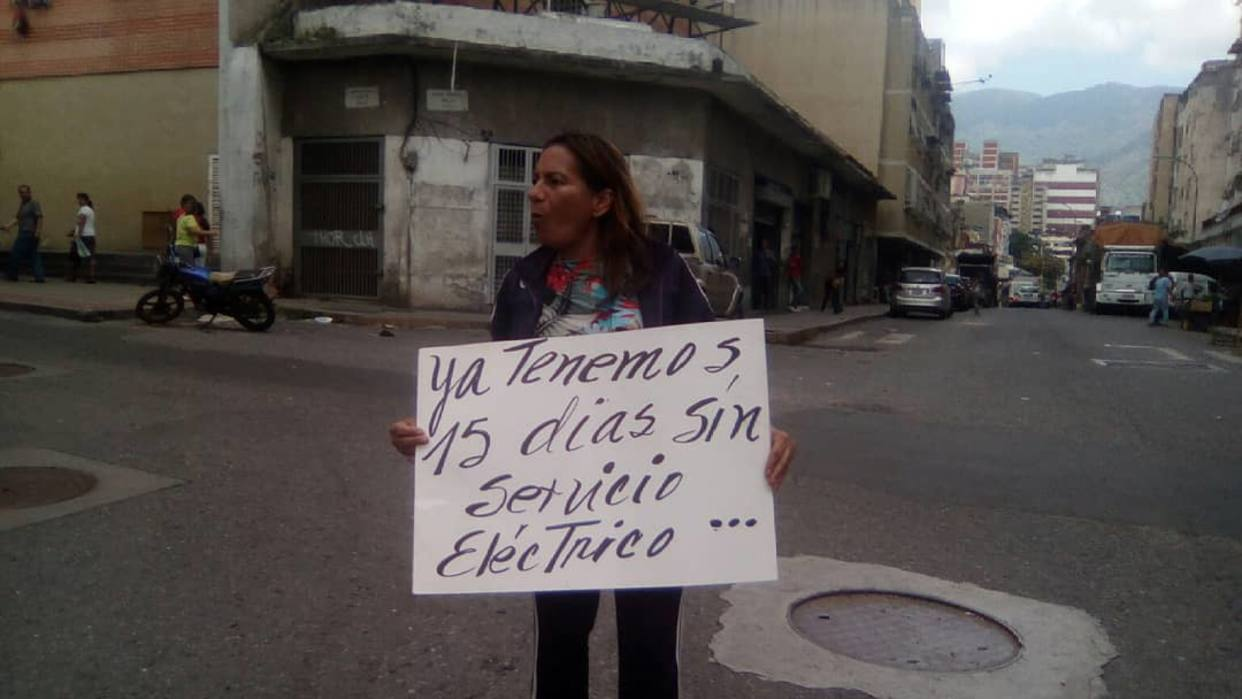
\includegraphics[width=300px]{37.jpg}%
\newline%
%
Habitantes del casco central de Santa Rosalía en Caracas, en Distrito Capital, trancaron las calles de la entidad por tener 15 días sin luz.%
\newline%
%
Los vecinos~de la comunidad trancaron el acceso de vehículos en la vía principal de la zona y exigen a Corpoelec una respuesta ante la falta del servicio.%
\newline%
%
Hasta ahora, el ente correspondiente no ha reportado la razón de la falla de electricidad en el sector.%
\newline%
%
\end{document}